\documentclass[urlcolor=blue,dvipsnames]{beamer}

\usepackage[utf8]{inputenc}
\usepackage{fancybox,fancyvrb}
\usepackage{environ}
\usepackage{tikz}
\hypersetup{colorlinks,linkcolor=,urlcolor=cyan}

\beamertemplatenavigationsymbolsempty
\setbeamertemplate{footline}[frame number]
\usetheme{Pittsburgh}

\newcommand\enumnum[1]{{\renewcommand{\insertenumlabel}{#1}%
      \usebeamertemplate{enumerate item} \,}}

\newcommand{\grad}{\nabla}
\newcommand{\ih}{\boldsymbol{\hat{\textbf{\i}}}}
\newcommand{\jh}{\boldsymbol{\hat{\textbf{\j}}}}
\newcommand{\vF}{\boldsymbol{\vec{\textbf{F}}}}
\newcommand{\Matlab}{\textsc{Matlab}}


\title{5.1 Linear mass-spring models}

\subtitle{a lesson for MATH F302 Differential Equations}

\author{Ed Bueler, Dept.~of Mathematics and Statistics, UAF}

\date{\tiny \today}


\begin{document}
\setbeamertemplate{itemize item}{$\bullet$}
\setbeamertemplate{itemize subitem}{$\circ$}


\begin{frame}
\titlepage

\centerline{\tiny for textbook: \, D. Zill, \emph{A First Course in Differential Equations with Modeling Applications}, 11th ed.}
%\color{green!40!blue}
\end{frame}


\begin{frame}{a good reason}

\begin{itemize}
\item in Chapter 4 we solved 2nd-order linear DEs
    $$a y'' + b y' + c y \stackrel{\ast}{=} g(t)$$
\item a good reason is that

\medskip
\centerline{\alert{anything that smoothly oscillates has $\ast$ for a model}}

    \begin{enumerate}
    \item a mass suspended on a spring oscillates up and down
    \item the current in an electrical circuit flows back-and-forth
    \item a pendulum swings back and forth
    \item the earth moves up and down in an earthquake
    \item magnetic field in a radio wave oscillates
    \item a drum-head vibrates
    \item a photon is
    \end{enumerate}

\item 5.1 and 5.3 slides cover \enumnum{1}--\enumnum{3}
\end{itemize}
\end{frame}


\begin{frame}{1st-order linear: no oscillation}

\begin{itemize}
\item why is 2nd-order needed for oscillation?
\item \emph{background assumption}: laws of nature are autonomous
\item 1st-order linear autonomous DEs cannot generate oscillation \small
\begin{align*}
y' &= a y + b \\
\int \frac{dy}{ay+b} &= \int dt \\
\frac{1}{a} \ln|ay+b| &= t+c \\
y(t) &= \frac{1}{a}\left(C e^{at} - b\right)
\end{align*}

\vspace{-3mm}
    \begin{itemize}
    \item solutions are \emph{always} growing/decaying exponentials
    \end{itemize}
\item 1st-order \emph{non}linear DEs would be nearly-linear for small solutions
\item summary: we expect oscillation models are 2nd-order
    \begin{itemize}
    \item we know examples: \footnotesize $y'' + y = 0 \iff y = c_1 \cos t + c_2 \sin t$
    \end{itemize}
\end{itemize}
\end{frame}


\begin{frame}{mass-spring model: the setup}

a specific set-up so that the equations are clear:
\begin{columns}
\begin{column}{0.6\textwidth}
\begin{itemize}
\small
\item hang spring from rigid support
    \begin{itemize}
    \item length $\ell$ and spring constant $k$
    \end{itemize}
\item choose mass $m$ and hook to the spring
\item it stretchs distance $s$ down to equilibrium position
\item mark length scale:
    \begin{itemize}
    \item $x=0$ is equilibrium position
    \item positive $x$ is downward
    \end{itemize}
\item $x$ is the displacement from additional stretch of the spring, i.e.~\emph{downward displacement of the mass from its equilibrium position}
\end{itemize}
\end{column}
\begin{column}{0.4\textwidth}
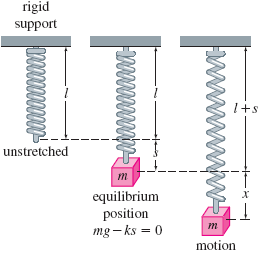
\includegraphics[width=\textwidth]{figs/mass-spring-setup}
\end{column}
\end{columns}
\end{frame}


\begin{frame}{Newton's law}

\begin{columns}
\begin{column}{0.65\textwidth}
\begin{itemize}
\item Newton's second law is $ma=F$
\item for our first mass-spring model:
        $$m \frac{d^2x}{dt^2} = mg - k (x+s)$$

\vspace{-3mm}
    \begin{itemize}
    \item but $mg=ks$ so
    $$\boxed{m \frac{d^2x}{dt^2} = - k x}$$
    \end{itemize}
\item ``Hooke's law'' $F_{spring} = -kx$ is a \emph{model} for how springs work
    \begin{itemize}
    \item not a bad model for small motions
    \item improved model in 5.3
    \end{itemize}
\item in practice:

\centerline{$k$ is \underline{determined} from $mg=ks$}
\end{itemize}
\end{column}
\begin{column}{0.35\textwidth}
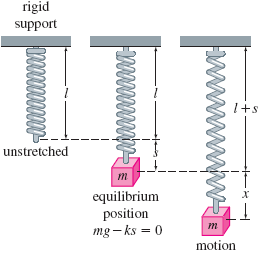
\includegraphics[width=\textwidth]{figs/mass-spring-setup}
\end{column}
\end{columns}
\end{frame}


\begin{frame}{(undamped) mass-spring solution}

\begin{itemize}
\item from last slide: $m \frac{d^2x}{dt^2} + k x = 0$
\item constant coefficient: substitute $x(t)=e^{rt}$ and get
    $$m r^2 + k = 0 \qquad \iff \qquad r = \pm \sqrt{\frac{k}{m}} i = \pm\, \omega i$$
\item \alert{$\omega = \sqrt{\frac{k}{m}}$}
\item general solution:
    $$x(t) = c_1 \cos(\omega t) + c_2 \sin(\omega t) \hspace{70mm}$$
\end{itemize}

\vspace{-20mm}
\hfill 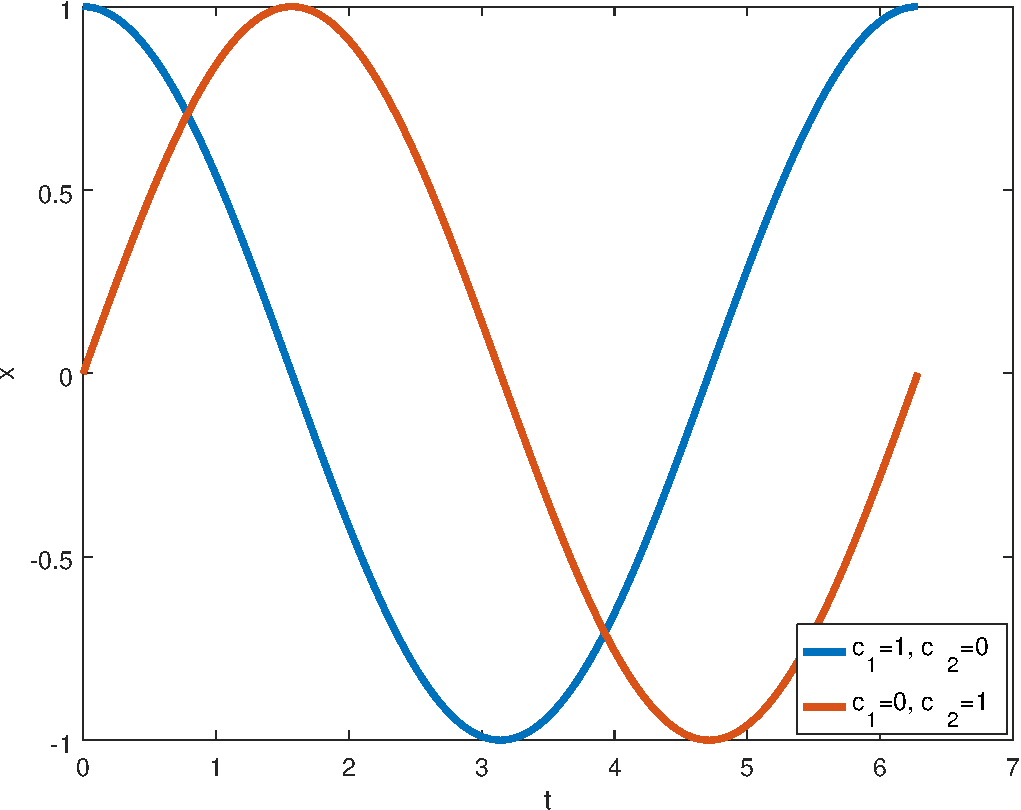
\includegraphics[width=0.45\textwidth]{figs/cossin}
\end{frame}


\begin{frame}{the meaning of $\omega$}

\begin{itemize}
\item general solution: $x(t) = c_1 \cos(\omega t) + c_2 \sin(\omega t)$
\item suppose $t$ is measured in seconds
\item then $\omega = \sqrt{\frac{k}{m}}$ is \alert{\emph{frequency of oscillation}} in radians per second
    \begin{itemize}
    \item units are correct because $\omega t$ must be in radians
    \end{itemize}
\item time \alert{$T = \frac{2\pi}{\omega}$} is \emph{period of oscillation}
    \begin{itemize}
    \item equation $\omega T=2\pi$ gives the smallest $T>0$ so that
        $$\cos(\omega T) = \cos(0) \quad \text{and} \quad \sin(\omega T) = \sin(0)$$
    \item \dots general solution has period $T$
    \end{itemize}
\end{itemize}
\end{frame}


\begin{frame}{exercise \#3 in \S5.1}

\begin{itemize}
\item ready for an exercise of the ``free undamped motion'' type:

\begin{quotation}
\noindent 3. A mass weighing 24 pounds, attached to the end of a spring, stretches it 4 inches.  Initially the mass is released from rest from a point 3 inches above the equilibrium position.  Find the solution for the motion.
\end{quotation}
\end{itemize}

\vspace{40mm}
\end{frame}


\begin{frame}{mass/weight stupidity}

\begin{itemize}
\item ``kilograms'' is the SI unit for \emph{mass} $m$
    \begin{itemize}
    \item $g=9.8 \,\text{m}/\text{s}^2$ is acceleration of gravity
    \item $mg$ is a force in newtons $N = \text{kg}\,\text{m}/\text{s}^2$
    \end{itemize}
\item ``pounds'' is a unit for \emph{force} $mg$
    \begin{itemize}
    \item it is a \emph{weight} not a mass
    \end{itemize}
\item ``slugs'' are a unit for \emph{mass} $m$
    \begin{itemize}
    \item old English system \dots
    \item and you need: $g=32 \,\text{ft}/\text{s}^2$
    \end{itemize}
\end{itemize}
\end{frame}


\begin{frame}{amplitude and phase of $x(t)$}

\begin{itemize}
\item for any $c_1,c_2$, this formula is a wave or oscillation:
    $$x(t) = c_1 \cos \omega t + c_2 \sin \omega t$$
\item what is its amplitude?
    \begin{itemize}
    \item only an easy question if either $c_1 =0$ or $c_2=0$
    \end{itemize}
\end{itemize}

\noindent {\color{Blue} Problem:} find  \emph{amplitude} $A$ and \emph{phase angle} $\phi$ so that
    $$\alert{x(t)} = c_1 \cos \omega t + c_2 \sin \omega t \alert{= A \sin(\omega t + \phi)}$$

\noindent {\color{Blue} Solution:} use $\sin(a+b) = \sin a \cos b + \cos a \sin b$ so
\begin{gather*}
A \sin(\omega t + \phi) = A \sin(\omega t) \cos\phi + A \cos(\omega t) \sin\phi \\
\implies \qquad \alert{c_1 = A \sin\phi, \, c_2 = A \cos \phi} \\
\implies \qquad \alert{A^2 = c_1^2 + c_2^2, \, \tan \phi = \frac{c_1}{c_2}}
\end{gather*}
\end{frame}


\begin{frame}{illustration}

\begin{itemize}
\item \emph{example:} graph $x(t) = A \sin(\omega t + \phi)$ for frequency $\omega=2.7$, amplitude $A=3.3$, and phase angle $\phi=0.3 \pi$
    \begin{itemize}
    \item period $T=2\pi/\omega = 2.51$
    \item $x(t) = 2.67 \cos(\omega t) + 1.94 \sin(\omega t)$
    \end{itemize}
\end{itemize}

\hfill 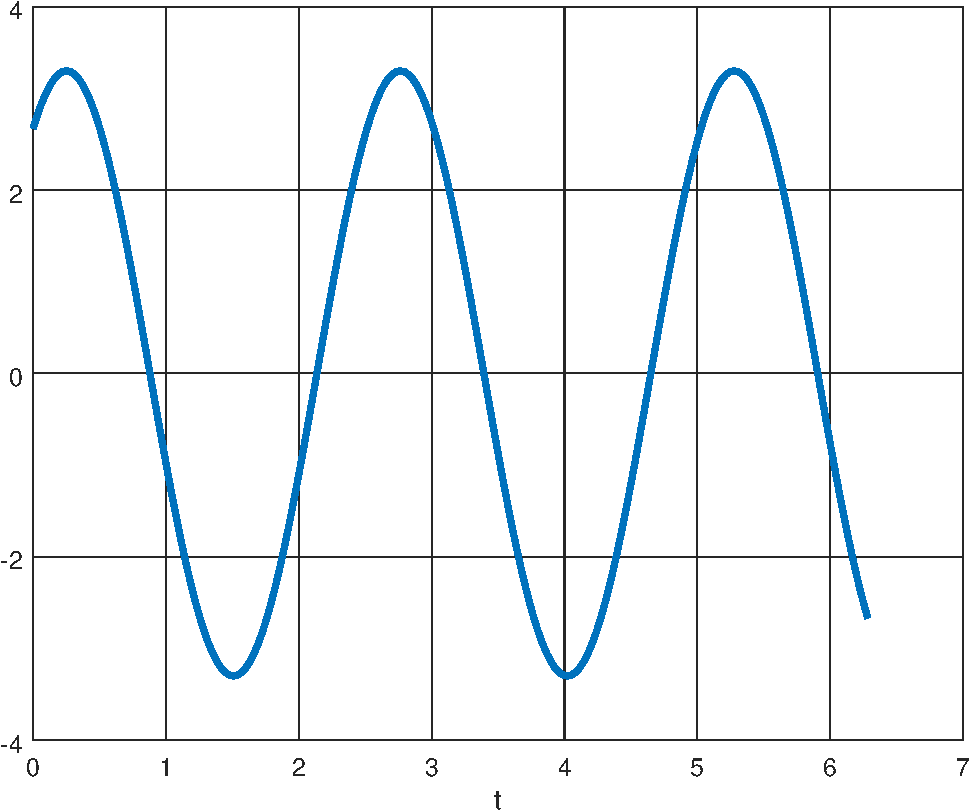
\includegraphics[width=0.6\textwidth]{figs/altwave}
\end{frame}


\begin{frame}{exercise \#6 in \S5.1}

\begin{itemize}
\item another exercise of the ``free undamped motion'' type:

\begin{quotation}
\noindent 6. A force of 400 newtons stretches a spring 2 meters.  A mass of 50 kilograms is attached to the end of the spring and is initially released from the equilibrium position with an upward velocity of 10 m/s.  Find the motion $x(t)$.
\end{quotation}
\end{itemize}

\vspace{40mm}
\end{frame}


\begin{frame}{damped mass-spring model}

\begin{columns}
\begin{column}{0.7\textwidth}
\begin{itemize}
\small
\item actual mass-springs don't oscillate forever
\item friction or drag is called ``damping''
    \begin{itemize}
    \item simple case: mass is surrounded by water or other fluid
    \end{itemize}
\item \emph{model}: damping is proportional to velocity
$$F_{\text{damping}} = - \beta v = - \beta \frac{dx}{dt}$$

\vspace{-2mm}
    \begin{itemize}
    \item $\beta > 0$ so damping force opposes motion
    \item same model as drag force for projectiles in sections 1.3, 3.1
    \end{itemize}
\item Newton's 2nd law again:
    $$\boxed{m \frac{d^2x}{dt^2} = - k x - \beta \frac{dx}{dt}} \qquad \text{or} \quad m x'' = -kx -\beta x'$$
\end{itemize}
\end{column}
\begin{column}{0.3\textwidth}
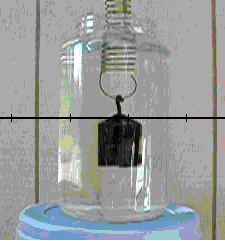
\includegraphics[width=1.1\textwidth]{figs/dampedmassspring}

\scriptsize movie at \href{https://bit.ly/2ThNjEk}{bit.ly/2ThNjEk}
%http://www.faculty.umassd.edu/adam.hausknecht/temath/TEMATH2/Examples/VideoImageSequences/DampedSpringModel.html
\end{column}
\end{columns}
\end{frame}


\begin{frame}{damped solution method}

\begin{itemize}
\item recall \emph{undamped} mass-spring model with $\alert{\omega = \sqrt{\frac{k}{m}}}$:
    $$m x'' = - k x \quad \iff \quad x'' + \omega^2 x = 0$$
\item new damped mass-spring model:
    $$m x'' = - k x - \beta x' \quad \iff \quad x'' + 2 \lambda x' + \omega^2 x = 0$$

\vspace{-2mm}
    \begin{itemize}
    \item $\displaystyle \alert{\lambda = \frac{\beta}{2m}}$

\vspace{1mm}
    \item auxiliary equation from $x(t)=e^{rt}$:
        $$r^2 + 2\lambda r + \omega^2=0$$

\vspace{-2mm}
    \item has roots:
        $$r = \frac{-2\lambda \pm \sqrt{4 \lambda^2 - 4 \omega^2}}{2} = -\lambda \pm \sqrt{\lambda^2 - \omega^2}=r_1,r_2$$

\vspace{-2mm}
    \item are $r_1,r_2$ distinct? real? complex?
    \end{itemize}
\end{itemize}
\end{frame}


\begin{frame}{exercise \#27 in \S5.1}

\begin{itemize}
\item exercise of the ``free damped motion'' type:

\begin{quotation}
\noindent 27. A 1 kilogram mass is attached to a spring whose constant is $16$ N/m.  The entire system is submerged in a liquid that imparts a damping force numerically equal to 10 times the instantaneous velocity.  Determine the equations of motion if the mass is initially released from rest from a point 1 meter below the equilibrium position.\end{quotation}
\end{itemize}

\vspace{40mm}
\end{frame}


\begin{frame}{slight variation comes out different}

\begin{quotation}
\noindent A 1 kilogram mass is attached to a spring whose constant is $16$ N/m.  The entire system is submerged in a liquid that imparts a damping force numerically equal to 6 times the instantaneous velocity.  Determine the equations of motion if the mass is initially released from rest from a point 1 meter below the equilibrium position.\end{quotation}

\vspace{50mm}
\end{frame}


\begin{frame}{damping cases}

$$\frac{d^2x}{dt^2} + 2 \lambda \frac{dx}{dt} + \omega^2 x=0$$

\begin{itemize}
\item \alert{\emph{undamped} if $\lambda = 0$}:
    $$x(t)=c_1 \cos(\omega t) + c_2 \sin(\omega t)$$
\item \alert{\emph{overdamped} if $\lambda^2-\omega^2 > 0$}: \hfill {\scriptsize $\boxed{r_1,r_2 = -\lambda \pm \sqrt{\lambda^2 - \omega^2}}$}
    $$x(t)=e^{-\lambda t} \left(c_1 e^{\sqrt{\lambda^2 - \omega^2}\, t} + c_2 e^{- \sqrt{\lambda^2 - \omega^2}\, t}\right)$$
\item \alert{\emph{critically damped} if $\lambda^2-\omega^2 = 0$}: \hfill {\scriptsize $\boxed{r_1=r_2 = -\lambda}$}
    $$x(t)=e^{-\lambda t} (c_1 + c_2 t)$$
\item \alert{\emph{underdamped} if $\lambda^2-\omega^2 < 0$}: \hfill {\scriptsize$\boxed{r_1,r_2 = -\lambda \pm \sqrt{\omega^2 - \lambda^2} i}$}
    $$x(t)=e^{-\lambda t} \left(c_1 \cos(\sqrt{\omega^2 - \lambda^2}\, t) + c_2 \sin(\sqrt{\omega^2 - \lambda^2}\, t)\right)$$
\end{itemize}
\end{frame}


\begin{frame}{damping cases pictured}

\begin{columns}
\begin{column}{0.45\textwidth}
\begin{itemize}
\item consider $m=1$, $k=4$
\item $\omega=\sqrt{\frac{k}{m}} = 2$:
    $$\frac{d^2x}{dt^2} + 2 \lambda \frac{dx}{dt} + 4 x=0$$
\item with initial values $x(0)=1,x'(0)=1$
\item picture cases $\lambda=1/4,2,5$
    \begin{itemize}
    \item recall $\lambda=\frac{\beta}{2m}$
    \item so $\beta = 1/2,4,10$
    \end{itemize}
\end{itemize}
\end{column}
\begin{column}{0.55\textwidth}
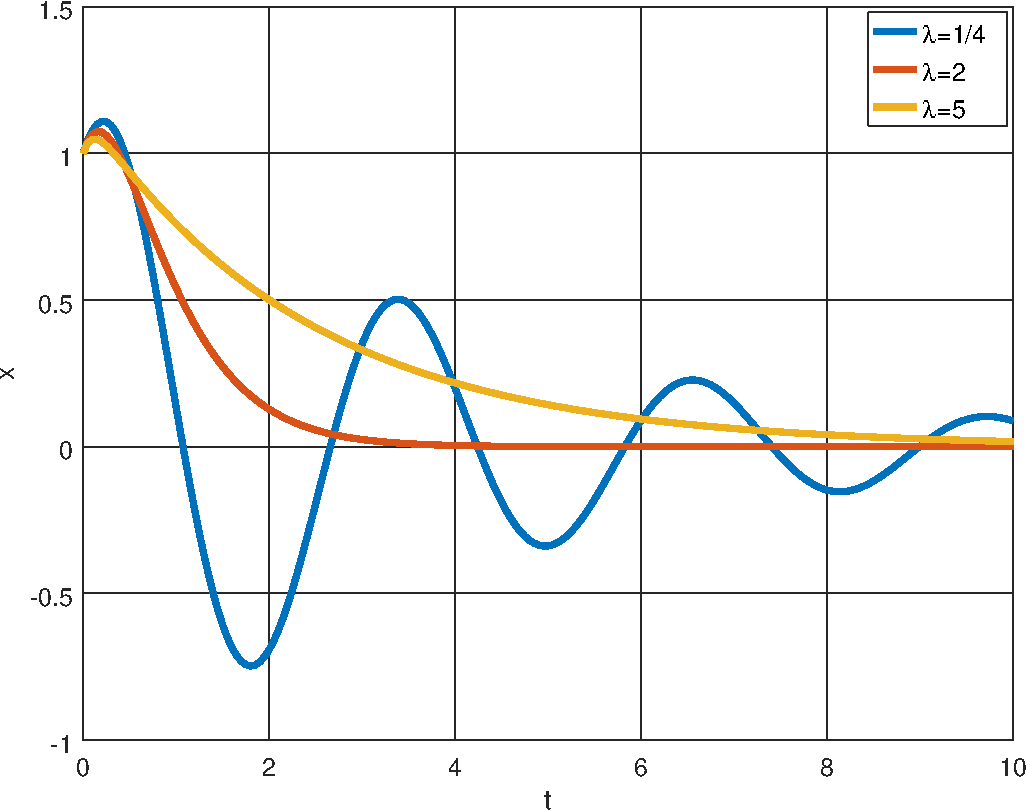
\includegraphics[width=1.03\textwidth]{figs/dampingcases}
\end{column}
\end{columns}
\end{frame}


\begin{frame}[fragile]
\frametitle{a plotting code: \texttt{massspringplot.m}}

\VerbatimInput[fontsize=\scriptsize]{../codes/massspringplot.m}
\end{frame}


\begin{frame}{example}

\noindent \emph{example:} solve the IVP
    $$mx'' = -kx - \beta x', \qquad x(0) = x_0, \, x'(0) = v_0$$
in the critically-damped case

\vspace{50mm}
\end{frame}


\begin{frame}{forced}

\begin{itemize}
\item the nonhomogeneous version is called a \emph{driven}, damped mass-spring where force $f(t)$ is applied to the mass:
    $$m \frac{d^2x}{dt^2} = - k x - \beta \frac{dx}{dt} + f(t)$$
\item equivalently, after dividing by $m$:
    $$\frac{d^2x}{dt^2} + 2 \lambda \frac{dx}{dt} + \omega^2 x=F(t)$$

\begin{minipage}[t]{0.5\textwidth}
\item a version of this model is a damped mass-spring formed by your car
    \begin{itemize}
    \item force is applied to the support and your car is the mass
    \end{itemize}
\end{minipage}
\end{itemize}

\vspace{-20mm}
\hfill 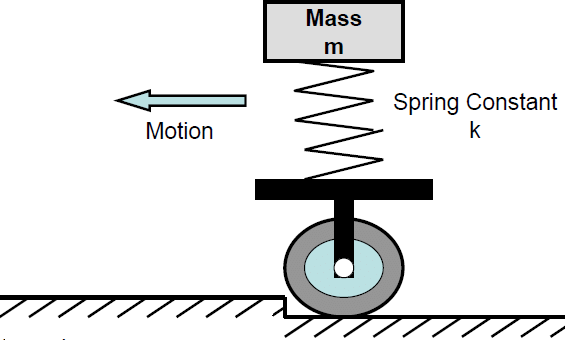
\includegraphics[width=0.4\textwidth]{figs/carbump}
\end{frame}


\begin{frame}{mass-spring DEs}

\begin{tabular}{r|c|c}
 & Newton's law: $ma=F$ & $\omega$ form \\ \hline \hline
\huge \strut \normalsize          undamped & $m \frac{d^2x}{dt^2} = - k x$ & $\frac{d^2x}{dt^2} + \omega^2 x=0$ \\ \hline
\huge \strut \normalsize            damped & $m \frac{d^2x}{dt^2} = - k x - \beta \frac{dx}{dt}$ & $\frac{d^2x}{dt^2} + 2 \lambda \frac{dx}{dt} + \omega^2 x=0$ \\ \hline
\huge \strut \normalsize \begin{tabular}{c} damped \\ and driven \end{tabular} & \small $m \frac{d^2x}{dt^2} = - k x - \beta \frac{dx}{dt} + f(t)$ & \small $\frac{d^2x}{dt^2} + 2 \lambda \frac{dx}{dt} + \omega^2 x=F(t)$ \\
\end{tabular}

\bigskip
\small
notes:
\begin{itemize}
\item $\omega=\sqrt{k/m}$, $\lambda = \beta / (2m)$, $F(t)=f(t)/m$
\item with driving force $f(t)$ the problem is \emph{nonhomogeneous}
\item you would solve the damped and driven problems by undetermined coefficients to find a particular solution (section 4.4)
\end{itemize}
\end{frame}


\begin{frame}{exercise \#43 in \S5.1}

\begin{quotation}
\noindent Solve the IVP
    $$\frac{d^2x}{dt^2} + \omega^2 x = F_0 \cos \gamma t, \qquad x(0)=0, \quad x'(0)=0$$
and compute $\displaystyle \lim_{\gamma\to\omega} x(t)$
\end{quotation}

\vspace{40mm}
\end{frame}


\begin{frame}{exercise \#43 pictured}

\begin{center}
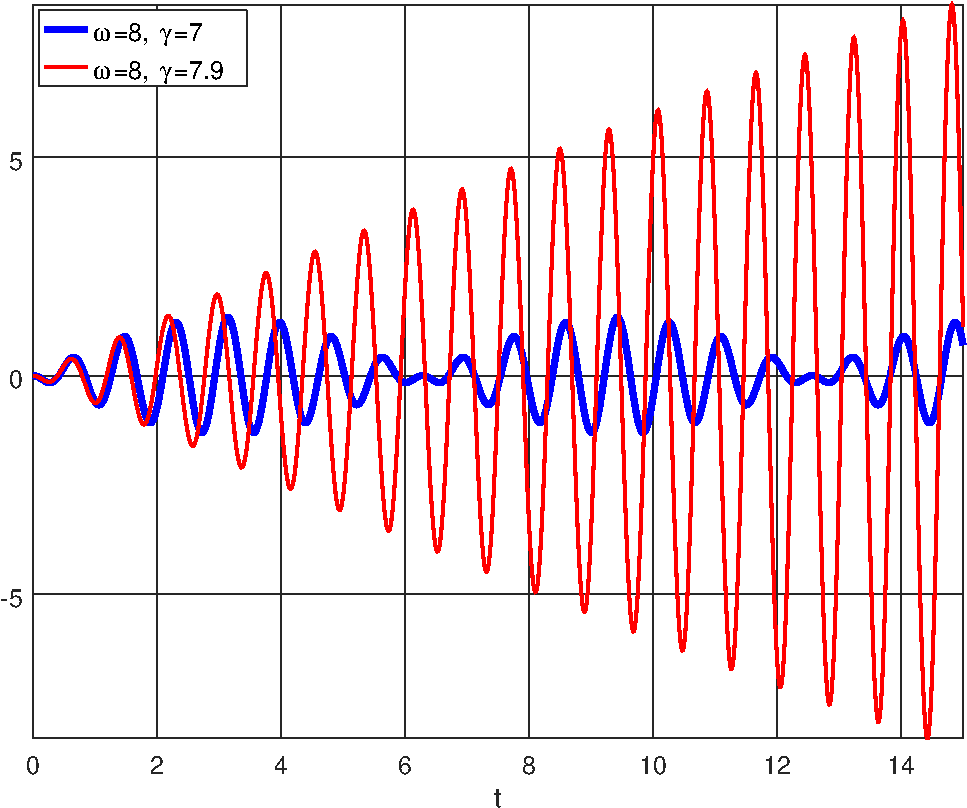
\includegraphics[width=0.7\textwidth]{figs/resonance}
\end{center}
%t=0:.01:15;
%plot(t,(10/(8^2-7^2))*(cos(8*t)-cos(7*t)),'b','linewidth',3.0)
%hold on,  plot(t,(10/(8^2-7.9^2))*(cos(8*t)-cos(7.9*t)),'r','linewidth',1.5)
%axis tight,  grid on,  xlabel t
%legend('\omega=8,\gamma=7','\omega=8,\gamma=7.9','location','northwest')

\begin{itemize}
\item idea: \alert{resonance} can occur in driven mass-spring systems
\end{itemize}
\end{frame}



\begin{frame}{RLC circuit}

\begin{itemize}
\item consider the electrical circuit:

\vspace{-3mm}
\hfill 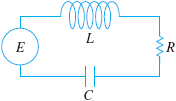
\includegraphics[width=0.45\textwidth]{figs/rlc-circuit}
\item has electical source ($E=E(t)$), an inductor ($L$), a resistor ($R$), and a capacitor ($C$)
\item a differential equation for the \emph{charge} $q$ is
    $$L \frac{d^2q}{dt^2} + R \frac{dq}{dt} + \frac{1}{C} q=E(t)$$
\item because $dq/dt = I$, a differential equation for the \emph{current} $I$ is
    $$L \frac{d^2I}{dt^2} + R \frac{dI}{dt} + \frac{1}{C} I=E'(t)$$
\end{itemize}
\end{frame}

\begin{frame}{circuit analogy}

\begin{tabular}{c|c}
mass-spring & electical circuit \\ \hline
mass $m$ & inductance $L$ \\
drag $\beta$ & resistance $R$ \\
spring constant $k$ & inverse of capacitance $1/C$ \\
applied driving force $f(t)$ & applied voltage source $E(t)$ \\
$mx''+\beta x'+k x = f(t)$ & $L q'' + R q' + \frac{1}{C} q=E(t)$
\end{tabular}

\bigskip
\begin{columns}
\begin{column}{0.7\textwidth}
\begin{itemize}
\item this is how radios are understood
    \begin{itemize}
    \item \emph{tuning a radio} means choosing the capacitance  $C$ to cause resonance at the frequency you want to hear from the input $E(t)$ from the antenna
    \end{itemize}
\item based on this idea there were \emph{analog computers} which used a configurable electical circuit to model mechanical motions
\end{itemize}
\end{column}
\begin{column}{0.4\textwidth}
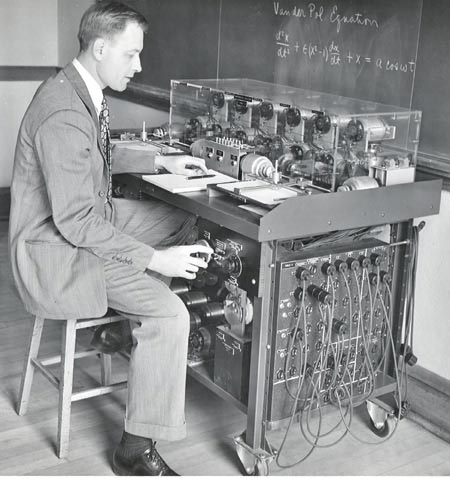
\includegraphics[width=0.95\textwidth]{figs/nordsieck-analog-computer}
\end{column}
\end{columns}
\end{frame}



\begin{frame}{expectations}

\begin{itemize}
\item just watching this video is \emph{not} enough!
     \begin{itemize}
     \item see ``found online'' videos at

     \centerline{\href{https://bueler.github.io/math302/week8.html}{\tt \color{cyan} bueler.github.io/math302/week8.html}}
     \item \emph{read} section 5.1 in the textbook
         \begin{itemize}
         \item material on ``double spring systems'' (p.~201) can be skipped
         \item while I discussed electrical circuits in these slides, I will not ask about it on quizzes or exams
         \end{itemize}
     \item \emph{do} the WebAssign exercises for section 5.1
     \end{itemize}
\end{itemize}
\end{frame}

\end{document}

